This chapter presents the requirement analysis and system architecture of the proposed Alzheimer's disease detection system. The system integrates 3D CNN-based local feature extraction with Vision-Transformer-based global attention, fuses the two, classifies the result, and explains it with 3D attribution methods --- all evaluated on the ADNI dataset under a leakage-free, subject-level protocol.

\section{Requirement Analysis}
Requirement analysis was conducted by reviewing:
\begin{itemize}
    \item Alzheimer's disease--related clinical and imaging literature
    \item Data characteristics and methodology from the reference papers
    \item Observed limitations (especially evaluation leakage) and performance metrics
\end{itemize}

\newpage
\subsection{Stakeholder Identification}
\begin{sloppypar}
\hyphenpenalty=50
\exhyphenpenalty=50
\hyphenchar\font=`\-
\begin{longtable}{|p{4cm}|p{5.5cm}|p{5cm}|}
\caption{Stakeholder Identification and Description}\\
\hline
\textbf{Stakeholder} & \textbf{Role in System} & \textbf{Interest}\\
\hline
Neurologists / Clinicians & Use the system's predictions and visual explanations to support diagnosis and decision-making. & Want accurate, reliable, and interpretable outputs that improve clinical confidence.\\
\hline
Researchers / Data Scientists & Develop, train, and evaluate the deep-learning models and ensure scientific validity. & Need transparent workflows, reproducible results, and honest performance insights.\\
\hline
Patients / Families & Indirect beneficiaries who receive improved diagnostic support through the system. & Prefer early detection, reduced uncertainty, and clinically meaningful outputs.\\
\hline
University Supervisors & Assess the methodology, implementation, and scientific contribution of the system. & Expect clear documentation, proper justification of methods, and strong research outcomes.\\
\hline
System Developers(Team) & Design, implement, and optimize the full pipeline from preprocessing to evaluation. & Need modular structure, maintainability, and reproducibility for future expansion.\\
\hline
\end{longtable}
\end{sloppypar}

In addition to the roles above, four practising clinicians gave \emph{informal} feedback on the system's outputs; their opinions are summarised in Table~\ref{tab:clin_feedback}. This was not a structured reader study: no blinding, fixed case set, or scoring protocol was used, so the table records stakeholder opinion and is \emph{not} evidence of clinical reliability --- which, as Section~\ref{sec:extval} shows, has not yet been demonstrated on external data. In particular, \textbf{Dr.\ Ziaur Rahman} (Physician \& Surgeon, \textbf{Comfort Diagnostic Center}) guided the labelling of the hospital scans used in the preliminary external-validation study (Section~\ref{sec:extval}); those labels were derived from routine radiology reports and are therefore treated as \emph{weak} labels rather than research-protocol diagnoses. These clinicians are key stakeholders for a future, properly designed evaluation of the system's cross-site applicability and the clinical value of its explainability outputs.

\begin{table}[H]
\centering
\caption{\textbf{Informal clinical stakeholder feedback.} Unstructured opinions of four practising clinicians on the system and its Grad-CAM explanations (not a blinded reader study).}
\label{tab:clin_feedback}
\begin{tabular}{|p{2.8cm}|p{2.6cm}|p{2.5cm}|p{3.2cm}|p{1.7cm}|}
\hline
\textbf{Name} & \textbf{Specialization} & \textbf{Clinical Reliability Opinion} & \textbf{Grad-CAM Clinically Relevant?} & \textbf{Helpful for Diagnosis?} \\
\hline
Dr.\ Ziaur Rahman & Physician \& Surgeon & Reliable & Yes, highly relevant & Yes \\
\hline
Dr.\ Abul Latif & Radiologist & Reliable & Yes, improves interpretability & Yes \\
\hline
Dr.\ Tania Kabir & Radiologist & Reliable & Partially relevant & Yes \\
\hline
Dr.\ Subir Chandra Das & Neurologist & Technically reliable & Yes, essential for model transparency & Yes \\
\hline
\end{tabular}
\end{table}

\subsection{Requirement Identification Methods}
\begin{itemize}
    \item Analysis of existing research papers (CNN, ViT, Swin, and hybrid AD classification)
    \item Comparative study of dataset characteristics and, critically, evaluation protocols
    \item Workflow observation from 3D preprocessing pipelines (reorientation, resampling, normalization)
    \item Evaluation metrics from the literature (accuracy, macro-F1, AUROC)
\end{itemize}
These sources provided the core requirements for the system functionality.

\subsection{Functional Requirements (FR)}
This is the list of Functional Requirements(FR):
\begin{sloppypar}
\hyphenpenalty=50
\exhyphenpenalty=50
\hyphenchar\font=`\-
\begin{longtable}{|p{3cm}|p{5cm}|p{6.5cm}|}
\caption{Table of Functional Requirements}\\
\hline
\textbf{Requirement ID} & \textbf{Functional Requirement} & \textbf{Description}\\
\hline
FR1 & MRI Input Handling & The system must accept 3D T1-weighted MRI volumes (NIfTI).\\
\hline
FR2 & Preprocessing Pipeline & Reorient to RAS, resample to isotropic spacing, foreground-crop, z-score normalize, and resize to a fixed tensor; augment during training.\\
\hline
FR3 & Subject-Level Splitting & Build stratified, subject-disjoint cross-validation folds so no subject's scans cross the train/test boundary.\\
\hline
FR4 & Feature Extraction & Provide 3D CNN, ResNet, ViT, and Swin backbones behind a common interface for extracting spatial/contextual features.\\
\hline
FR5 & Classification Module & Classify binary CN-vs-AD and three-class CN/MCI/AD using a shared softmax head.\\
\hline
FR6 & Explainable AI & Generate Grad-CAM, Integrated-Gradients, and attention-rollout overlays for interpretability.\\
\hline
FR7 & Performance Evaluation & Compute accuracy, macro/weighted-F1, per-class precision/recall, ROC-AUC, and confusion matrices at scan and subject level.\\
\hline
\end{longtable}
\end{sloppypar}

\subsection{Non-Functional Requirements (NFR)}
Below is a list of Non-Functional Requirements(NFR):
\begin{sloppypar}
\hyphenpenalty=50
\exhyphenpenalty=50
\hyphenchar\font=`\-
\begin{longtable}{|p{3cm}|p{5cm}|p{6.5cm}|}
\caption{Table of Non-Functional Requirements}\\
\hline
\textbf{Requirement ID} & \textbf{Non-Functional Requirement} & \textbf{Description}\\
\hline
NFR1 & Accuracy & Achieve an \emph{honest} subject-level result that clearly exceeds the majority-class baseline and is reported with fold-wise variance, rather than an inflated leakage-based number.\\
\hline
NFR2 & Reliability & Produce consistent results across folds; report mean\,$\pm$\,std, not a single lucky split.\\
\hline
NFR3 & Performance & Support GPU-accelerated training within a 16\,GB VRAM budget; inference is fast.\\
\hline
NFR4 & Reproducibility & Fixed seeds, saved configs and splits, and one-command regeneration of results and figures.\\
\hline
NFR5 & Usability & Clinician-friendly, interpretable heatmap outputs.\\
\hline
NFR6 & Maintainability & Modular pipelines for data, models, training, evaluation, and explainability.\\
\hline
NFR7 & Security & Use only anonymized, ethically approved data; protect MRI privacy.\\
\hline
\end{longtable}
\end{sloppypar}

\section{System Overview / Architecture}
The proposed system follows a modular deep-learning pipeline that combines convolution-based local feature extraction with transformer-based global attention. It preprocesses raw 3D MRI, extracts local and global features through a dual-path network, fuses the representations, classifies the Alzheimer's status, and explains the decision --- all under a subject-level evaluation that keeps the reported accuracy honest.

\subsection{High-Level Architecture}
The system consists of five major modules:\\
\textbf{1. Data Acquisition and Curation Module} \\
This module ingests 3D T1-weighted MRI volumes from ADNI, indexes them by image ID, attaches the CN/MCI/AD labels, and removes off-pipeline scans. It builds the stratified, subject-level cross-validation folds that guarantee leakage-free evaluation.

\noindent\textbf{2. Preprocessing Module} \\
This component reorients volumes to RAS, resamples them to 1.5\,mm isotropic spacing, crops the foreground, applies z-score intensity normalization over non-zero voxels, and resizes to a fixed cubic tensor ($96^3$ for all binary runs and the three-class ViT; $128^3$ for the three-class CNN and Swin; see Appendix~\ref{app:repro}). Deterministic outputs are cached; training augmentation (flips, affine, noise, intensity jitter) is applied on the fly.

\noindent\textbf{3. Feature Extraction and Classification Module} \\
\begin{itemize}
    \item \textbf{CNN backbone} --- 3D DenseNet-121 (local features).
    \item \textbf{Pretrained CNN} --- MedicalNet 3D ResNet (transfer-learning baseline).
    \item \textbf{Transformer backbones} --- 3D ViT and Swin (global features).
    \item \textbf{Hybrid} --- CNN$+$ViT with late-concatenation or cross-attention fusion.
    \item \textbf{Classifier} --- a shared dropout$+$linear$+$softmax head over the backbone/fused features.
\end{itemize}

\noindent\textbf{4. Explainability Module (XAI)} \\
This module produces Grad-CAM / Grad-CAM++ / Score-CAM heatmaps, Integrated-Gradients and SmoothGrad attributions, occlusion sensitivity, and attention rollout for the transformer branch, overlaid on the MRI for clinical interpretation.

\noindent\textbf{5. Model Evaluation and Reporting Module} \\
This component computes accuracy, macro/weighted-F1, sensitivity, specificity, ROC-AUC, and confusion matrices at both scan and subject level, and aggregates the five folds into mean\,$\pm$\,std summaries with comparison plots.

\newpage
\subsection{Detailed Design Diagrams}
Figure~\ref{fig:block} shows the high-level block diagram of the system, Figure~\ref{fig:flow} the end-to-end experimental flowchart, and Figure~\ref{fig:hybrid} the hybrid 3D CNN--ViT fusion architecture.
\begin{figure}[H]
    \centering
    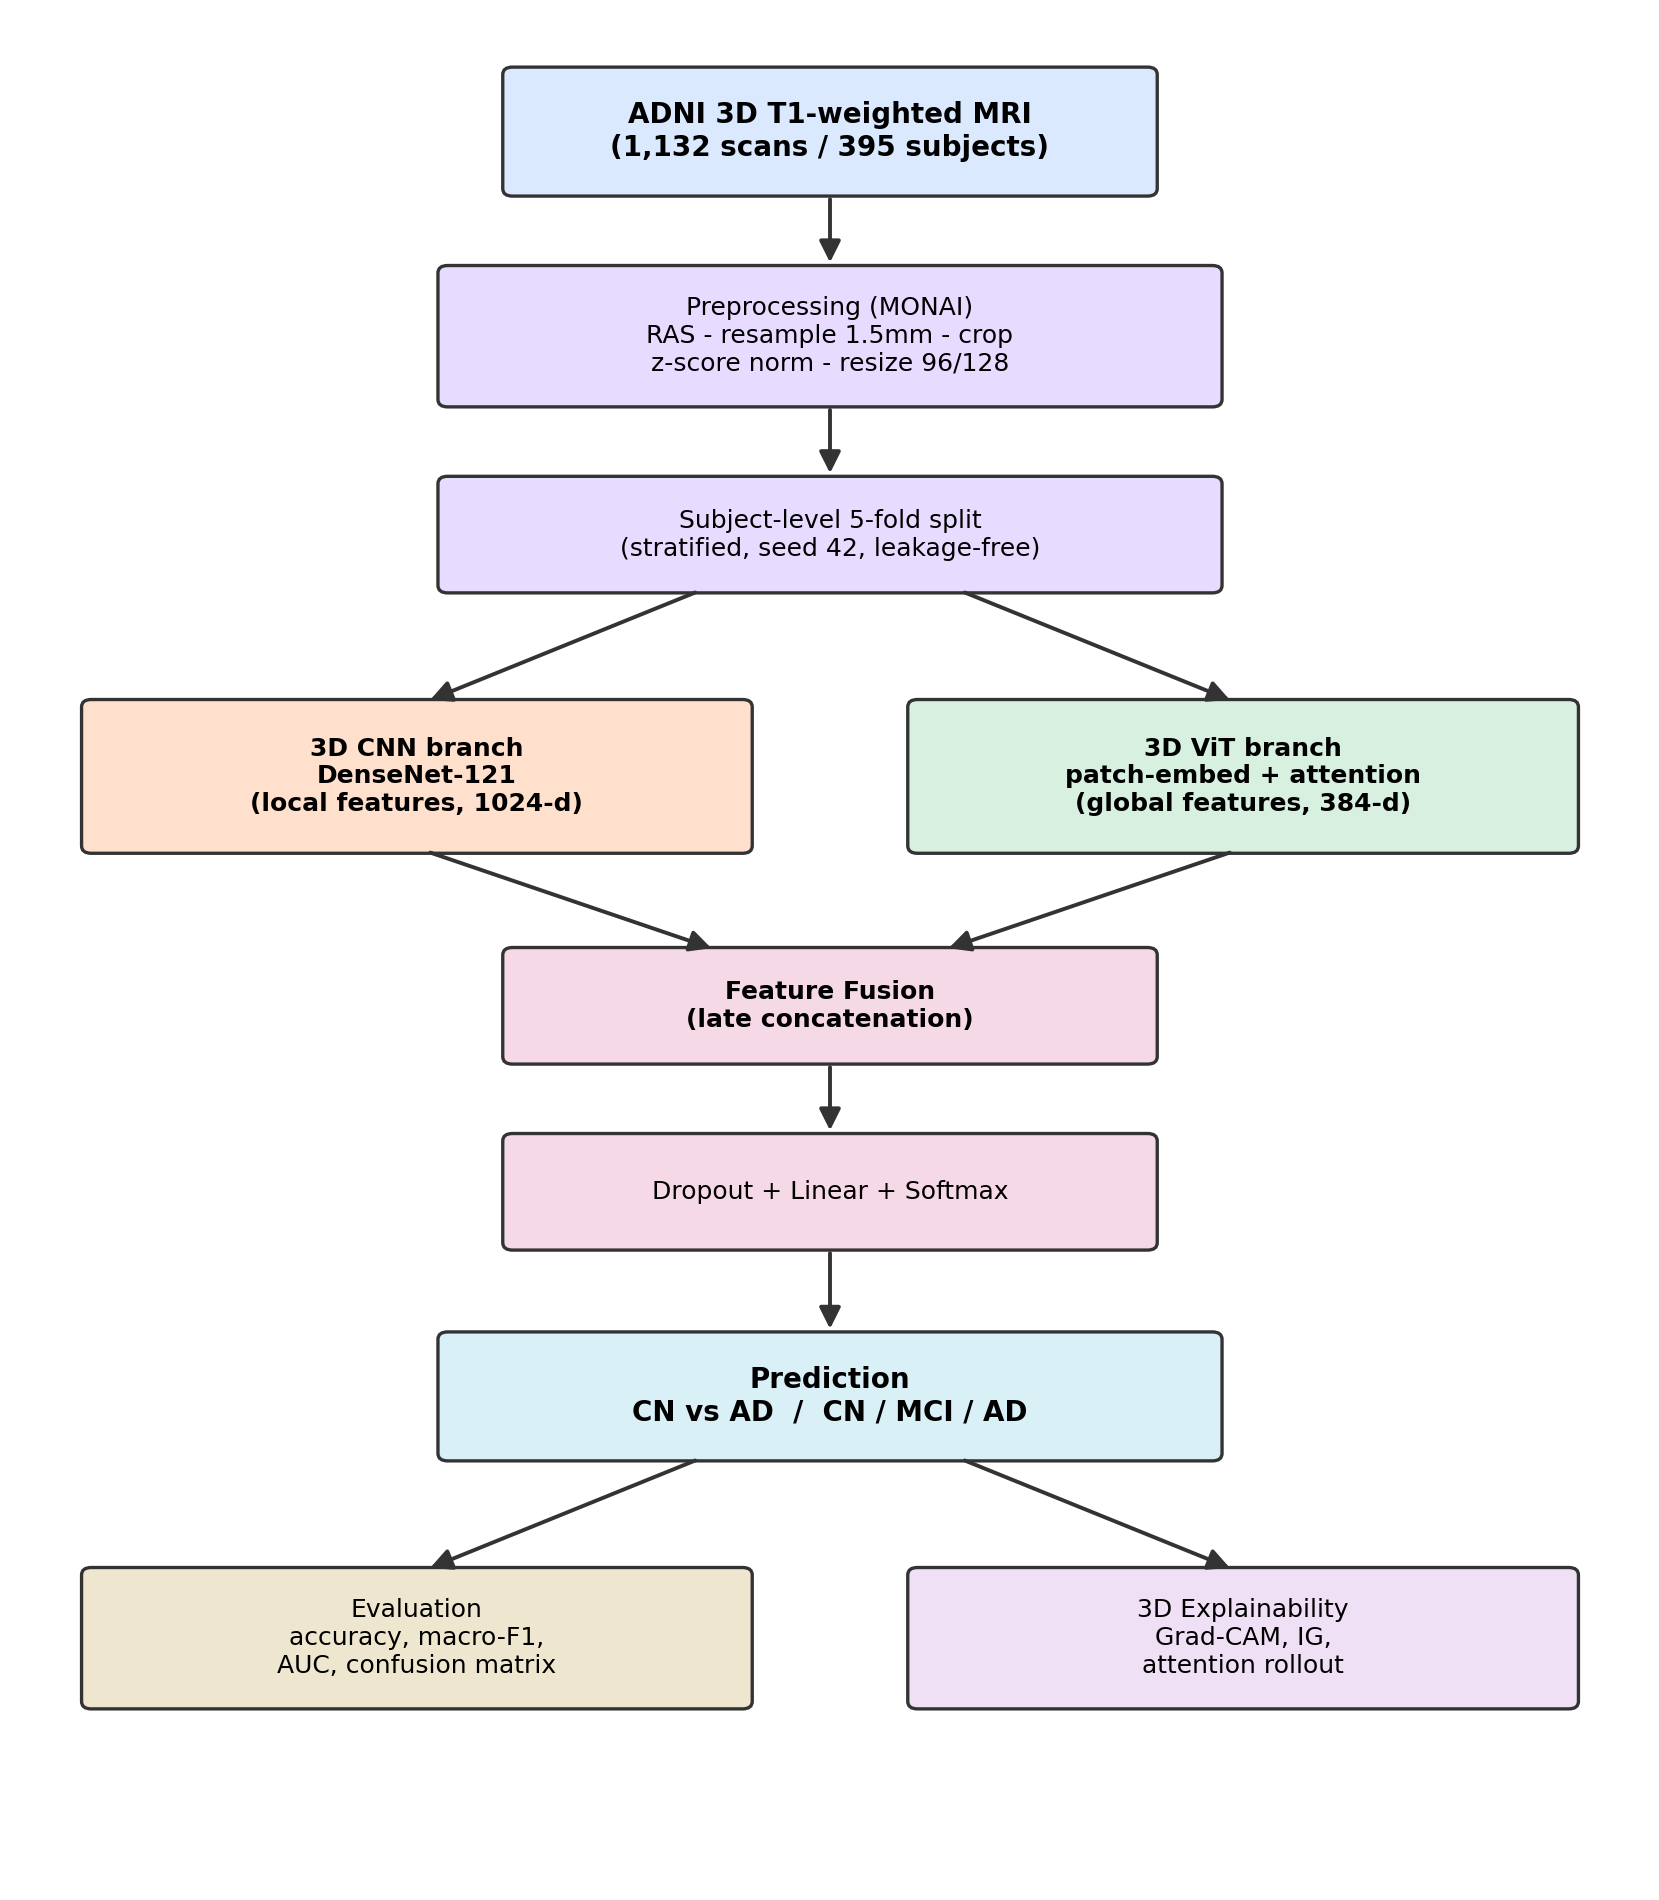
\includegraphics[width=11cm]{Images/arch_block_diagram.png}
    \caption[System block diagram]{\textbf{System block diagram.} High-level view of the proposed dual-branch 3D CNN--ViT system on ADNI.}
    \label{fig:block}
\end{figure}
\begin{figure}[H]
    \centering
    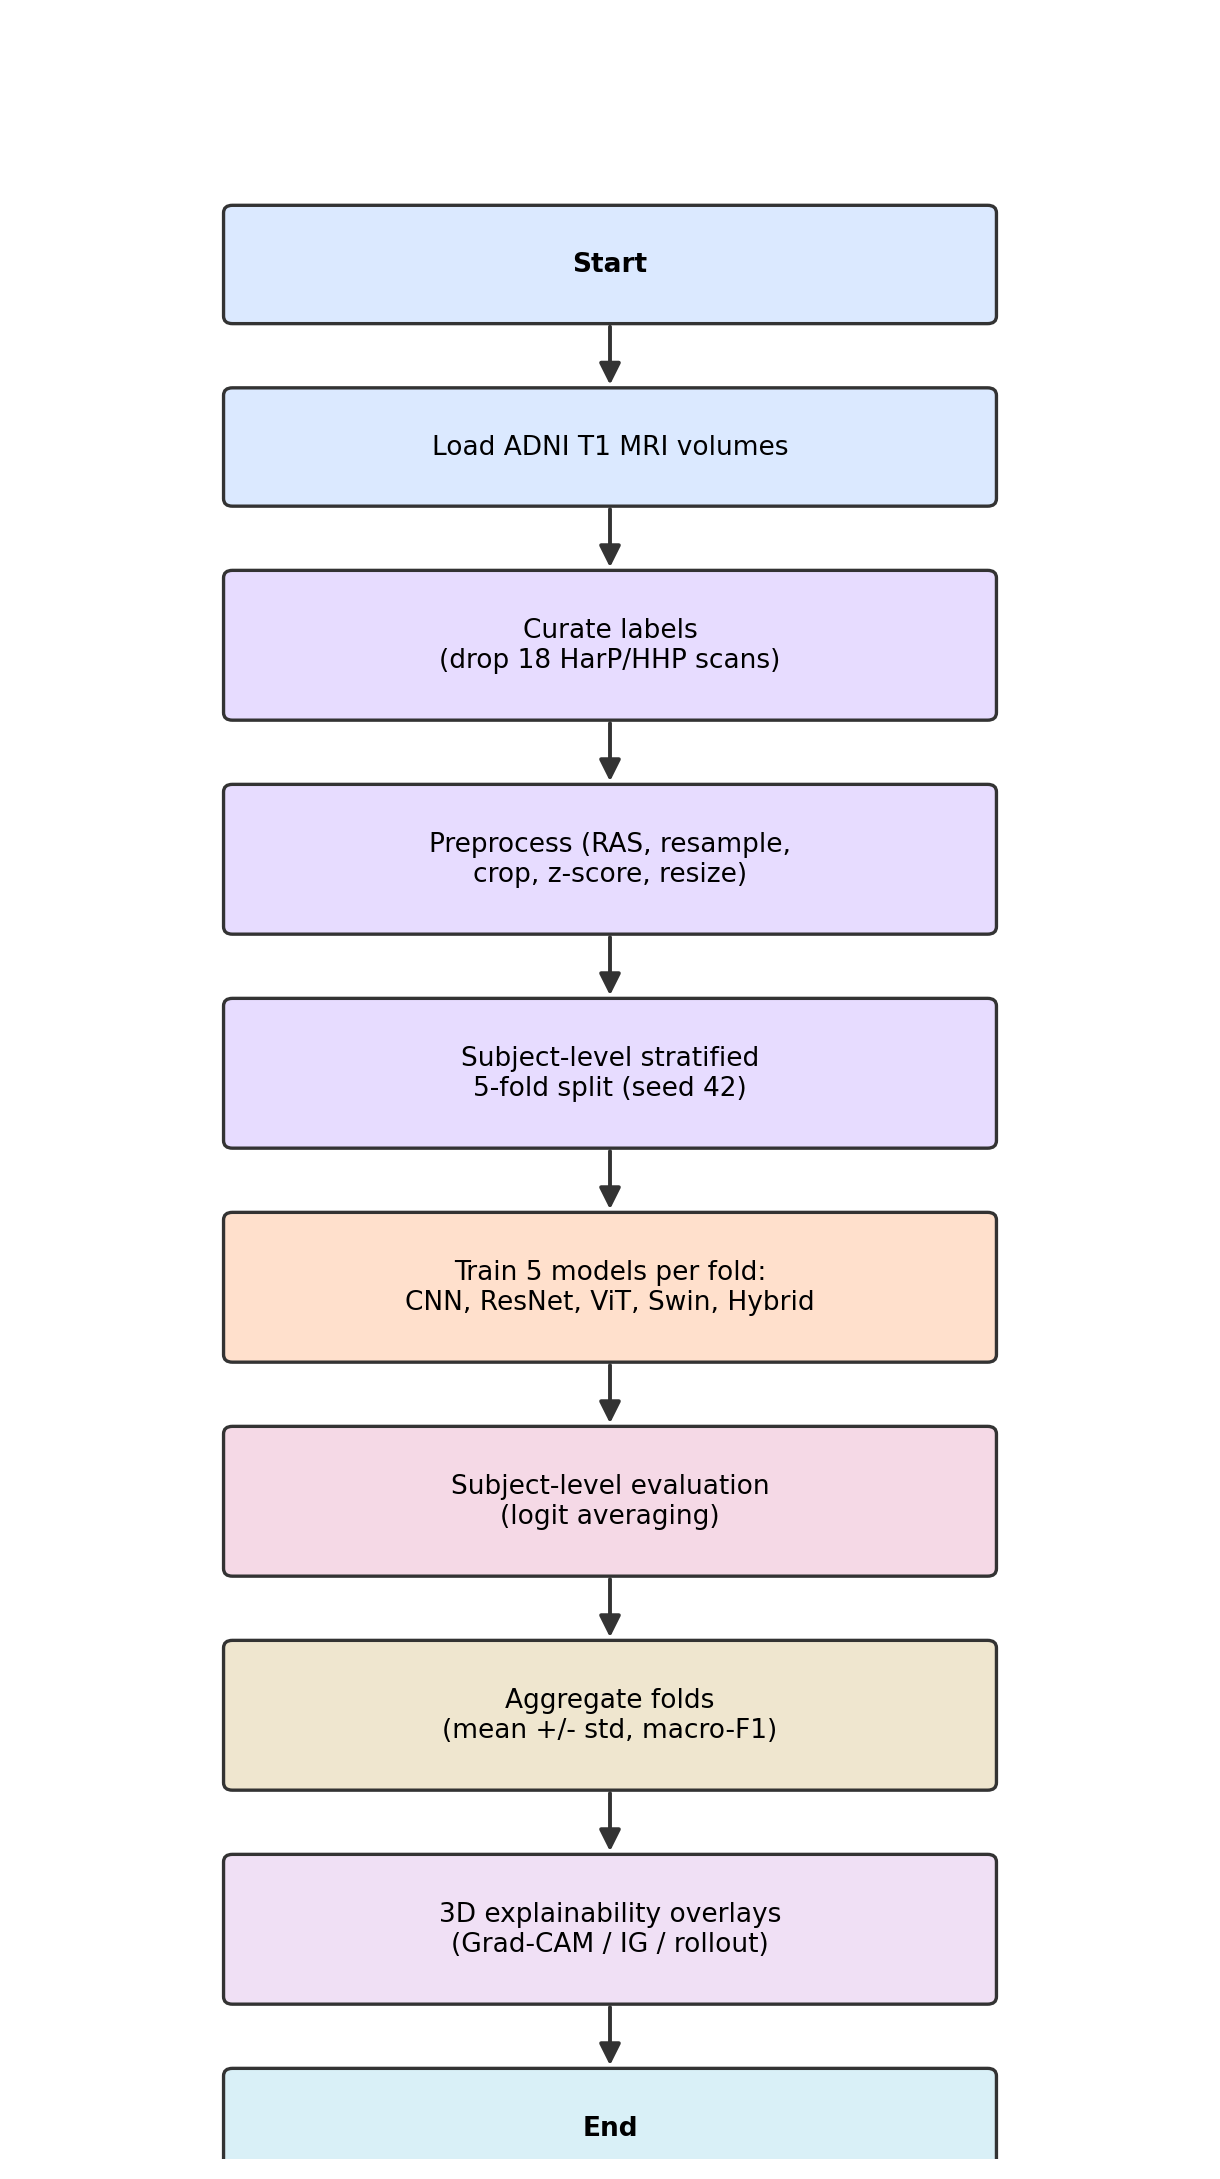
\includegraphics[width=9cm]{Images/arch_flowchart.png}
    \caption[Experimental flowchart]{\textbf{Experimental flowchart.} End-to-end pipeline from ADNI ingestion to subject-level evaluation and explainability.}
    \label{fig:flow}
\end{figure}
\begin{figure}[H]
    \centering
    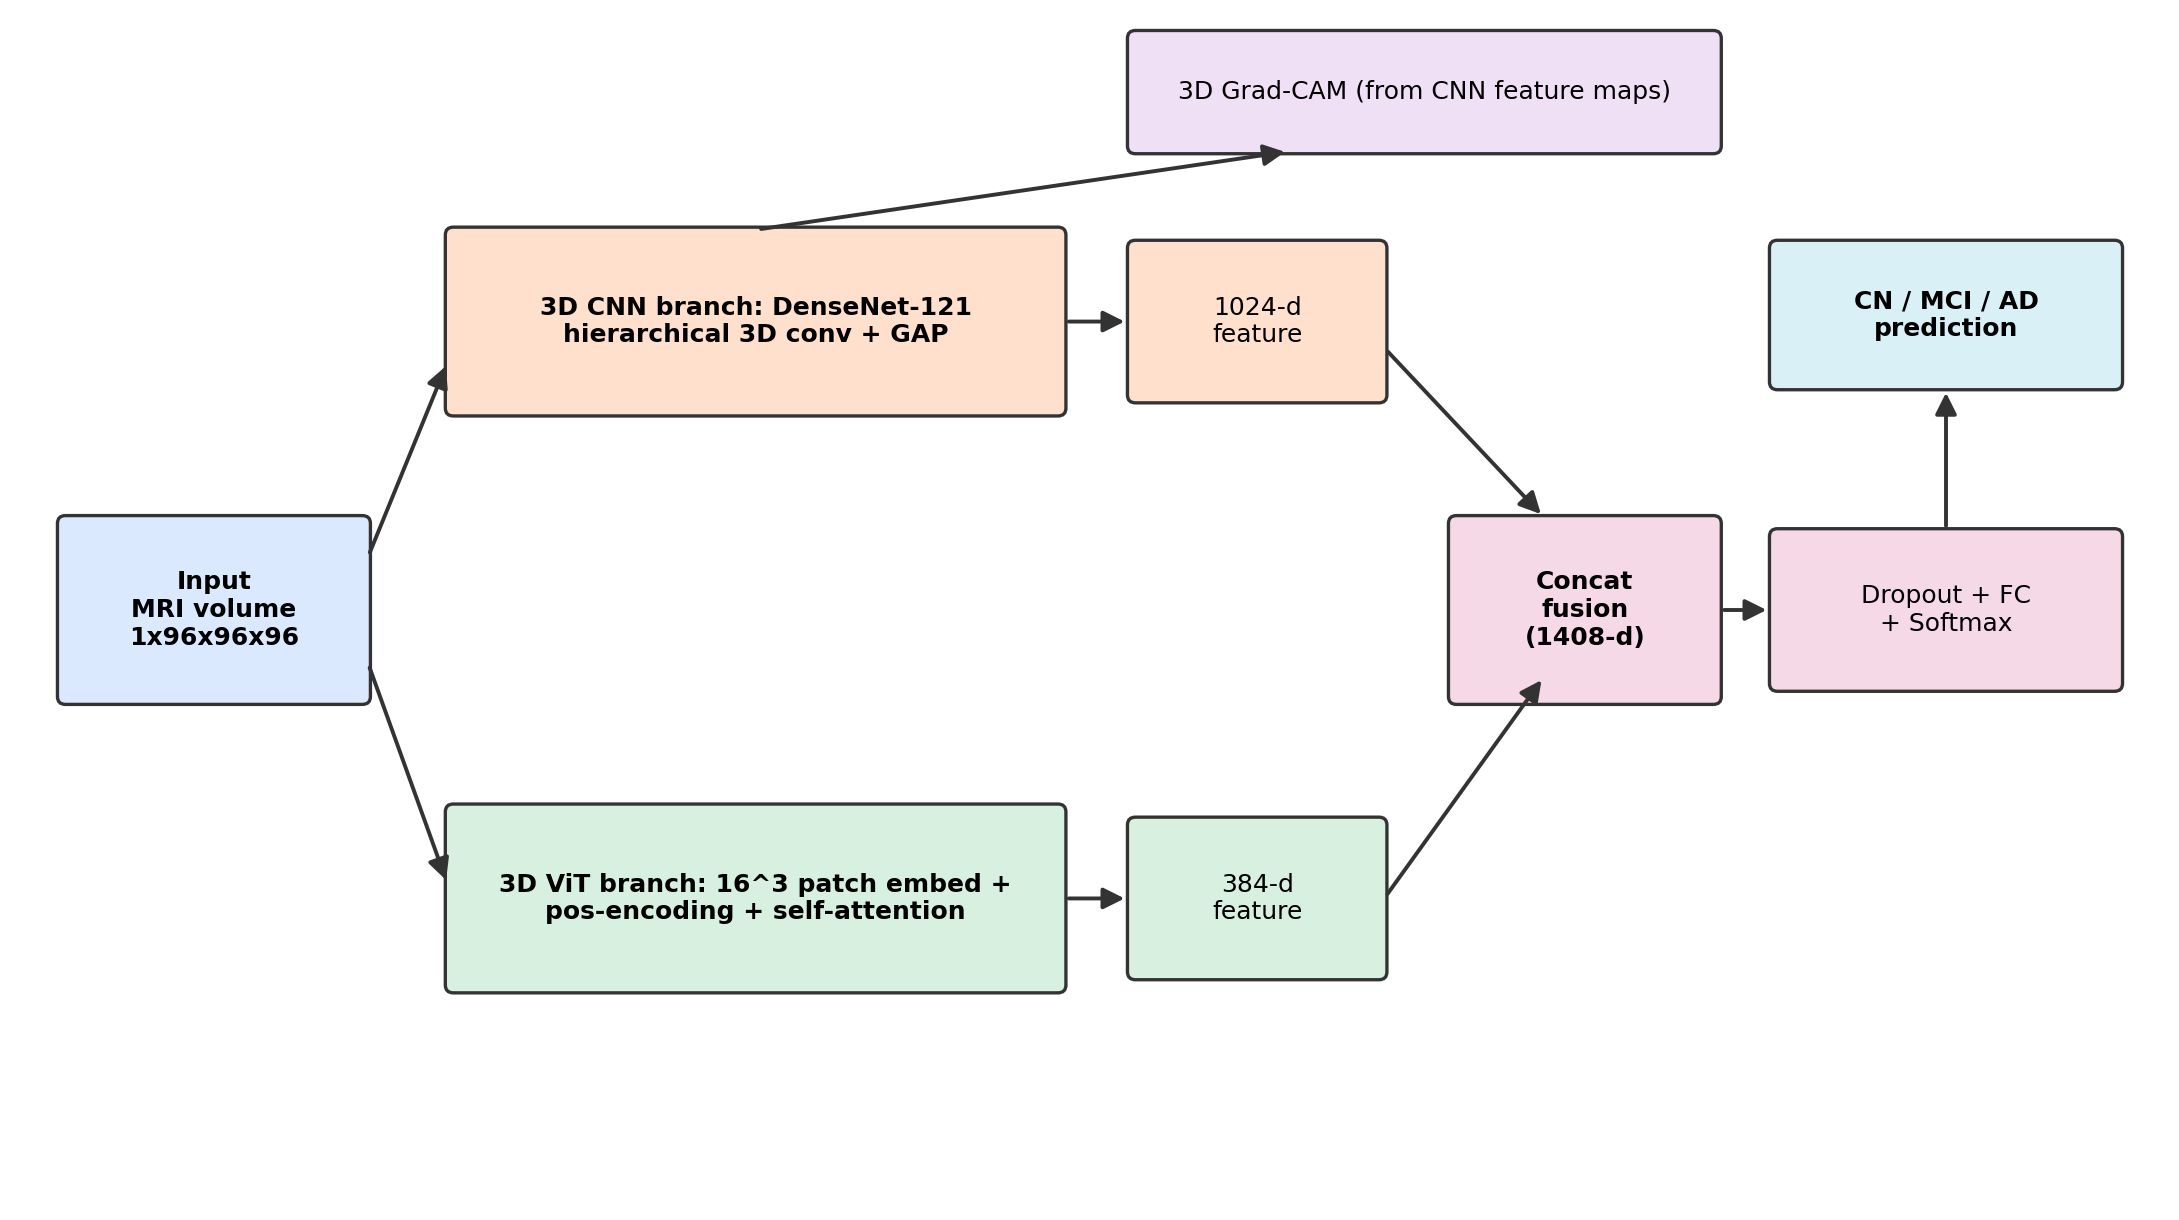
\includegraphics[width=15cm]{Images/arch_hybrid.png}
    \caption[Hybrid fusion architecture]{\textbf{Hybrid fusion architecture.} The 3D CNN (DenseNet) branch extracts local texture features (1024-D) and the 3D ViT branch extracts global contextual features (384-D) from the \emph{same} input volume; the two vectors are combined by late concatenation (1408-D) and passed to a shared dropout$+$linear classifier head with softmax. Grad-CAM is computed from the CNN branch for explainability.}
    \label{fig:hybrid}
\end{figure}

\subsection{Design Alternatives and Rationale}
Several architectural alternatives were considered. A standalone 3D CNN captures local spatial features strongly but has a limited receptive field for long-range relationships. A standalone 3D Vision Transformer models global context well but is data-hungry and, as the experiments confirm, underperforms when trained from scratch on a few hundred subjects. A 2D slice-based model is easy and fast but discards volumetric context and, worse, invites patient-level data leakage.\\
Weighing performance potential, resource cost, and --- crucially --- evaluation honesty, the hybrid 3D CNN--3D ViT architecture was selected: the CNN branch supplies fine local anatomical detail and the inductive bias the transformer lacks, while the ViT branch adds global reasoning across the whole volume. Fusing the two, combined with 3D Grad-CAM, yields a design that is modular, efficient on a single 16\,GB GPU, and --- as Chapter~\ref{cha:results} shows --- statistically tied for the best binary result with the standalone CNN, which is itself an informative outcome of a fair comparison against its own single-model baselines.

\section{Pseudocode for Proposed 3D CNN--ViT Hybrid Model}
\begin{algorithm}[H]
\caption{Hybrid 3D CNN--ViT Classification Pipeline}
\begin{algorithmic}[1]
\Require MRI\_volume (Raw 3D Brain Scan)
\Ensure Prediction $\in$ \{CN, AD\} (binary) or \{CN, MCI, AD\} (three-class)

\State MRI $\gets$ LoadVolume(MRI\_volume)
\State MRI $\gets$ Preprocess(MRI)
\Statex \quad ReorientRAS();\ ResampleIsotropic();\ CropForeground()
\Statex \quad ZScoreNormalize();\ Resize()
\Statex \quad \textit{// skull-stripping / MNI registration optional (ablation)}
\State Volume $\gets$ Standardize(MRI)

\State CNN\_features $\gets$ DenseNet3D(Volume) \Comment{local, 1024-d}
\State ViT\_features $\gets$ ViT3D(Volume) \Comment{global, 384-d}

\State Fused $\gets$ Concatenate(CNN\_features, ViT\_features)
\State Output $\gets$ FullyConnected(Dropout(Fused))
\State Prediction $\gets$ Softmax(Output)

\State Heatmap $\gets$ GradCAM3D(CNN\_features)
\State \textbf{return} Prediction, Heatmap
\end{algorithmic}
\end{algorithm}

\section{Summary}
This chapter presented the system design underlying the proposed framework. It specified the stakeholders, functional and non-functional requirements (including the explicit requirement of an \emph{honest}, subject-level accuracy target), and a five-module architecture spanning data curation, 3D preprocessing, the CNN/ViT/Swin/hybrid feature-extraction bank, explainability, and evaluation. The block, flowchart, and hybrid-architecture diagrams illustrated component interaction and data flow, and the pseudocode clarified the operational path from a raw MRI volume to a classified, explained prediction. This blueprint guides the methodology and experiments that follow.
